% -----------------------------------------------
% TP1 — Composição Musical Algorítmica (UFMG, 2026)
% Based on the official ISMIR 2026 LaTeX template (ismir.sty).
%
% Compile:  pdflatex main && bibtex main && pdflatex main && pdflatex main
%       or  tectonic main.tex
% Figures and tables come from scripts/run_analysis.py.
% -----------------------------------------------

\documentclass{article}
\usepackage[T1]{fontenc}
\usepackage[utf8]{inputenc}
\usepackage{ismir} % camera-ready mode: shows the author, no line numbers
\usepackage{amsmath,cite,url}
\usepackage{graphicx}
\usepackage{booktabs}
\usepackage{color}

% This is a course assignment, not an ISMIR paper: drop the proceedings
% header and replace the venue in the copyright box.
\fancyhead[l]{}
\makeatletter
\renewcommand{\permission}{%
  \begin{figure}[b]{%
    \footnotesize
    {
\includegraphics[alt={CC-BY License},height=0.45cm]{cc_by.pdf}}
    \vskip -.45cm
    \begin{spacing}{1.1}
      \hskip 1.5cm \copyright \hskip .1cm \authorname.
      Licensed under a Creative Commons Attribution 4.0 International License (CC BY 4.0).
      \textbf{Attribution:} \authorname,
      ``\removelinebreaks{\@title}'', course assignment (TP1),
      \textit{AI for Music Generation}, UFMG, 2026.
    \end{spacing}
    }
  \end{figure}
}
\makeatother

\title{Bach Chorale Melodies with Variable-Order\\ Markov Chains: Coherence versus Memorization}

\oneauthor
  {Lucas Junqueira Carvalhido}
  {Universidade Federal de Minas Gerais (UFMG)\\\texttt{lucasjunqueiracarvalhido@gmail.com}}

\def\authorname{L. J. Carvalhido}

\sloppy

\begin{document}

\maketitle

\begin{abstract}
We present an end-to-end symbolic melody generator based on $n$-th order Markov chains, constrained to the style of the soprano lines of J.\,S.~Bach's four-part chorales. Melodies are represented as sequences of (pitch, duration) events, transposed to C, and transition probabilities are estimated by maximum likelihood from 195 major-mode chorales. Generation uses backoff to lower orders for unseen contexts, a temperature parameter, and start/end tokens that let the model learn openings and cadences. We quantify the classic trade-off of the model order by measuring, over 50 melodies per order, how much of the output is copied verbatim from the corpus. Order 1 copies almost no 6-event span (2\%) and sounds aimless, while order 4 copies 85\% of its 6-grams and reproduces runs of 17 events on average. Order 2 is a good compromise and is our default. Code, MIDI files and audio renderings are available at \url{https://github.com/Lucas-Junqueira/TP1_IA_Musica}.
\end{abstract}

\section{Introduction}\label{sec:introduction}

Markov chains are among the oldest methods of algorithmic composition: the next musical event is drawn from a probability distribution conditioned on the $n$ previous ones. They need no hand-written rules or fitness function, as the probabilities can be counted directly from a corpus, and the model order $n$ gives a single, interpretable control over how closely the output follows that corpus.

We adopt a fixed stylistic constraint: the generated pieces are monophonic melodies in the style of the \emph{soprano lines of Bach chorales}. This repertoire is homogeneous (short hymn phrases, mostly stepwise motion, phrase endings marked by fermatas), large enough to estimate low-order statistics, and readily available in the \texttt{music21} corpus~\cite{cuthbert2010}. The goal of this work is to build the full pipeline, from corpus to audio, and to measure how the order trades randomness for memorization.

\section{Related Work}\label{sec:related}

Brooks et al.~\cite{brooks1957} trained Markov chains of orders 1 to 8 on 37 hymn tunes and already observed the behavior we revisit here: low orders produce random-sounding melodies, and high orders reproduce fragments of the training tunes. Ames~\cite{ames1989} surveys the use of Markov processes as a compositional model. Pachet's \emph{Continuator}~\cite{pachet2003} uses variable-order Markov models for real-time interaction in the style of a performer, backing off to shorter contexts when a long one has not been seen, which is the strategy we use. Later work addresses the memorization problem directly: Markov constraints~\cite{pachet2011} make generation steerable, and Papadopoulos et al.~\cite{papadopoulos2014} bound the length of verbatim copies from the corpus. Broader context can be found in the surveys of Fernández and Vico~\cite{fernandez2013} and Nierhaus~\cite{nierhaus2009}.

\section{Method}\label{sec:method}

\textbf{Corpus and representation.} We iterate over the 371 chorales of \texttt{music21}, select the soprano part by name (falling back to the top part), and estimate the key of the full four-part score. Only the 195 chorales analyzed as major are kept, and each is transposed to C by the smallest interval ($-6$ to $+5$ semitones), so the model learns scale degrees instead of absolute keys, reducing sparsity. Each melody becomes a sequence of events $e = (\text{MIDI pitch}, \text{duration in quarter notes})$, e.g. $(67, 1.0)$, with pitch 0 for rests. Tied notes are merged, fermatas are ignored, grace notes are dropped and consecutive rests are fused. The corpus contains 10{,}066 events; 67\% of durations are quarter notes. Every melody is padded with $n$ \textsc{start} tokens and one \textsc{end} token, so openings and cadences are learned as regular transitions.

\textbf{Training.} For each order $k=0,\dots,n$ we count how often each event follows each context of the $k$ previous tokens. Transition probabilities are the normalized counts (maximum likelihood): $P(e \mid c) = N(c, e) / N(c)$. Nothing is set by hand.

\textbf{Generation.} Starting from $n$ \textsc{start} tokens, the next event is sampled from the distribution of the longest known context; if a context of order $n$ was never observed, the model backs off to order $n-1$, and so on down to order 0 (unconditional event frequencies). A temperature $T$ reshapes the distribution as $p_i \propto N(c,e_i)^{1/T}$: $T<1$ favors frequent transitions and $T>1$ flattens the distribution. Generation stops when \textsc{end} is sampled or after 64 events. Because cadential contexts (e.g. a long tonic) often lead straight to \textsc{end}, \textsc{end} is masked during the first 24 events; when a context has \textsc{end} as its only continuation, this also triggers backoff. Finally, the last note is lengthened to complete the last 4/4 bar, and the melody is written as MIDI (piano, 80\,BPM) and rendered to audio with FluidSynth and the FluidR3 General MIDI soundfont. The hyperparameters are the order $n$, the temperature $T$ and the random seed, so the same configuration produces different pieces with different seeds.

\section{Experiments and Results}\label{sec:results}

\textbf{Setup.} For each order $n \in \{1,2,3,4\}$ we generated 50 melodies (seeds 0--49, $T=1$). To measure memorization we index every contiguous span of the corpus with a suffix automaton~\cite{blumer1985}, which gives, for each position of a generated melody, the longest span ending there that occurs verbatim in a single chorale. From it we compute (i) the fraction of generated 6-grams found in the corpus and (ii) the longest copied run. We use 6-grams because an order-$n$ model only emits $(n{+}1)$-grams seen in training, so shorter $n$-grams would be trivially copied for orders 3 and 4.

\begin{figure}[t]
  \centering
  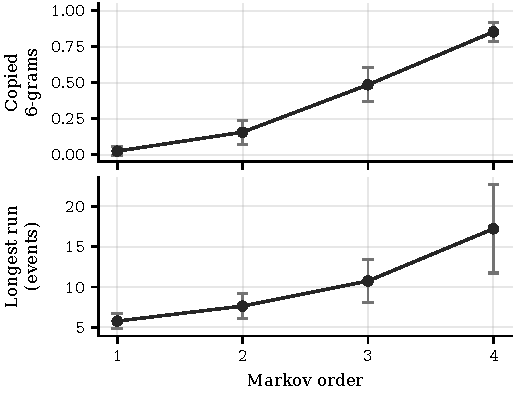
\includegraphics[alt={Copied 6-grams and longest copied run versus Markov order},width=\columnwidth]{figures/metrics_by_order.pdf}
  \caption{Memorization versus Markov order (mean $\pm$ s.d.\ over 50 melodies, $T=1$).}
  \label{fig:order}
\end{figure}

\begin{table}[t]
  \centering
  \small
  \setlength{\tabcolsep}{4pt}
  \begin{tabular}{ccccc}
    \toprule
    Order & Contexts & $H$ (bits) & Copied 6-grams & Longest run \\
    \midrule
    1 & $152$ & $3.04$ & $0.02 \pm 0.03$ & $5.8 \pm 0.9$ \\
    2 & $1044$ & $2.11$ & $0.16 \pm 0.08$ & $7.6 \pm 1.6$ \\
    3 & $2696$ & $1.31$ & $0.48 \pm 0.12$ & $10.7 \pm 2.6$ \\
    4 & $4432$ & $0.70$ & $0.85 \pm 0.07$ & $17.2 \pm 5.5$ \\
    \bottomrule
  \end{tabular}
  \caption{Model sparsity and memorization by Markov order. Contexts: distinct contexts seen in training; $H$: mean conditional entropy of the next event. The last two columns are mean $\pm$ s.d.\ over 50 melodies ($T = 1$); longest run is the longest span, in events, copied verbatim from one chorale.}
  \label{tab:results}
\end{table}


\textbf{Order trade-off.} \tabref{tab:results} and \figref{fig:order} show the expected monotonic trend. As the order grows, the number of distinct contexts multiplies (152 to 4{,}432) while each context is seen fewer times, so the conditional entropy drops from 3.0 to 0.7 bits: at order 4 the next event is nearly determined by the corpus. The fraction of copied 6-grams rises from 2\% to 85\%, and the longest verbatim run triples (5.8 to 17.2 events, i.e. several phrases of a single chorale). All 50 melodies were distinct at every order, so the copying is of fragments, not of whole chorales. Backoff was rare (0.02 to 0.24 times per melody), and only triggered by the minimum-length mask.

\textbf{Temperature.} At order 2, lowering $T$ to 0.5 raises the copied 6-grams from 15\% to 36\%, while $T=1.5$ and $T=2$ lower it to 11\% and 10\%. Temperature thus offers a finer control over the same trade-off than the order does.

\textbf{Listening examples.} We rendered six pieces, available in the \texttt{outputs/audio/} folder of the repository and named \texttt{ord\{n\}\_temp\{T\}\_seed\{s\}}. \emph{Order 1, seed 1} wanders over 16 semitones, places rests in the middle of phrases and uses a chromatic C$\sharp$ with no harmonic purpose: locally plausible, globally directionless. \emph{Order 2, seeds 1--3} are mostly stepwise, with recognizably chorale-like phrases closed by long notes or rests. Seed 1 ends with the cadence D--C on the tonic; seed 2 ends on F, without closure; seed 3 drifts to an A-minor cadence (G$\sharp$--A) and contains a 9-beat rest copied from a chorale with an instrumental interlude. \emph{Order 3, seed 1} is a coherent descending line from C5 to C4 ending on a 2--1 cadence. \emph{Order 4, seed 1} sounds most like Bach, but its longest run is 12 events copied from a single chorale, i.e. a quarter of the piece. We therefore use \textbf{order 2} as default: it keeps local voice-leading and cadential idioms while copying fewer than one in six 6-grams.

\section{Discussion and Future Work}\label{sec:discussion}

The model sees only the last $n$ events, so it has no notion of phrase length, meter position or long-term form. Phrases have irregular lengths, and 34--46\% of the melodies reach the 64-event limit without sampling \textsc{end}, so they stop without a cadence. Because events carry no beat position, pickups and barlines are not aligned, and the last-note padding is only a cosmetic fix. Key analysis also errs on some chorales, which explains endings outside C. Future work includes adding the metric position to the state, imposing a four-bar phrase structure, modeling all four voices to recover the harmony, and bounding copy length with Markov constraints~\cite{pachet2011,papadopoulos2014}.

\bibliography{refs}

\end{document}
